% LLNCS macro package for Springer Computer Science procedings;
% Version 2.20 of 2017/10/04
%\documentclass[runningheads]{llncs}
\documentclass[]{llncs} % Using this for now

\usepackage{graphicx} % Still need this for when you add images later
\usepackage{amsmath}  % For math (e.g., the n in N-person)
\usepackage{hyperref} % For clickable links
\hypersetup{
    colorlinks=true,
    linkcolor=blue,
    citecolor=green,
    urlcolor=magenta
}
\usepackage{appendix} % For appendix section


\begin{document}

\title{Navigating the N-Person Prisoner's Dilemma: From the Tragic Valley
  to the Collaborative Hill}
% \titlerunning{N-Person IPD: Tragedy Valley to Reciprocity Hill} % Uncomment if classictype is runningheads

\author{Chris Tcaci and Chris Huyck\inst{1}}
% \authorrunning{C. Tcaci} % Uncomment if classictype is runningheads
\institute{Middlesex University, London NW4 4BT UK\\
\email{M00674787@mdx.ac.uk} \and \email{c.huyck@mdx.ac.uk} \\
\url{https://cwa.mdx.ac.uk/chris/chrisroot.html}
}

\maketitle

%undone are they agents or players

\begin{abstract}
  The N-Person Iterated Prisoner's Dilemma (N-IPD) is an excellent
  environment to explore collaboration.

  This paper investigates how agent-based learning models navigate this complex social dilemma. We demonstrate that simple reinforcement learning agents consistently fall into a "Tragedy Valley" of mutual defection in standard N-IPD neighbourhood interaction models. However, by enhancing agents with contextual awareness of their local environment and employing adaptive Multi-Agent Reinforcement Learning (MARL) algorithms like Hysteretic-Q and Wolf-PHC, high levels of sustained cooperation (over 85\%) can be achieved. Furthermore, we explore the fundamental impact of interaction structure, contrasting the neighbourhood model with a pairwise interaction model where agents play repeated 2-player games. The pairwise model, by enabling direct reciprocity, facilitates a climb towards a "Reciprocity Hill," where cooperation is more readily established and maintained. Our findings highlight the critical roles of agent cognition, learning algorithms, and interaction structure in fostering cooperation in multi-agent systems.

\keywords{N-Person Prisoner's Dilemma \and Agent-Based Modelling \and Reinforcement Learning \and Emergence of Cooperation \and Tragic Valley \and Collaborative Hill \and Multi-Agent Systems.}
\end{abstract}

\section{Introduction}
\label{sec:introduction}

The Prisoner's Dilemma (PD) serves as a foundational paradigm in game
theory, illustrating the conflict between individual rational
self-interest and mutually beneficial collective action
\cite{Axelrod}.  In its simplest form, two individuals, unable to
communicate, must independently choose whether to cooperate or
defect. While mutual cooperation yields a good outcome for both, each
player has an individual incentive to defect, leading to a suboptimal
outcome if both choose to do so. The Iterated Prisoner's Dilemma
(IPD), where the game is played repeatedly, opens the door for
cooperation to emerge through strategies based on reciprocity, as
famously demonstrated by Axelrod's tournaments where Tit-for-Tat
proved remarkably successful \cite{Axelrod}.

However, many real-world social and economic dilemmas—ranging from
managing common-pool resources to international climate agreements and
team collaborations—involve more than two interacting parties. The
N-Person Iterated Prisoner's Dilemma (N-IPD) generalizes the IPD to
scenarios with $n$ participants \cite{Hamburger1973, Hardin1971}.


This paper will first provide a brief background on the N-IPD and
relevant learning approaches (Section \ref{sec:background}). It then
describes



\section{Background and Related Work}
\label{sec:background} % Renamed for clarity, was sec:litreview

This section briefly reviews key concepts from game theory, focusing on the
N-Person Prisoner's Dilemma (N-IPD), and introduces the Agent-Based Modelling
(ABM) and Multi-Agent Reinforcement Learning (MARL) approaches relevant to this
paper. 

\subsection{The Prisoner's Dilemma}
The canonical version of the Prioner's Dilemma was presented by
Axelrod and Hamilton \cite {Axelrod}.  There are two prisoners
and they are given the option to turn the other in.  So both have
the option to collaborate, and not turn the other in, or defect.
That is each has a choice {\it C} or {\it D}.  Each is given a reward
based on their decision and the decision of the other.  If they both
collaborate they both are given $R$, a reward.  If both defect they
are $P$, a punishment.  If one defects, and the other collaborates,
the defector is given $T$, a temptation, and the collaborator is given
$S$, a sucker's payoff.  

\begin {table} [ht]
\begin{center}
\begin {tabular}{c | c | c |}
\hline
& $R_{1,2}$ &  $T_1 S_2$ \\
\hline
& $T_2 S_1$ &  $P_{1,2}$ \\
\hline
\end {tabular}
\caption {The table represents the outcomes for the four scenarios when
  two prisoners vote.  When both collaborate, both get $R$, and when
  both defect, both get $P$.  When one collaborates and one defects,
  the defector gets $T$ and the collaborator gets $S$ payoff.}
\label {tabPayoff}
\end {center}
\end {table}

Axelrod and Hamilton restrict the values so that equations \ref {restrict1}
and \ref {restrict2} are followed.  A standard set of values is $T=5$, $R=3$,
$P=1$ and $S=0$.

\begin{equation}\label{restrict1}
T > R > P > S 
\end{equation}
\begin{equation}\label{restrict2}
R > (S + T) / 2
\end{equation}

The IPD merely plays the tournament over and over.  This gives the agents
a chance to develop their own policy.  


\subsection{The N-Person Prisoner's Dilemma (N-IPD)}

The Iterated Prisoner's Dilemma (IPD) serves as a critical model for understanding cooperation. While Axelrod's work highlighted the success of strategies like Tit-for-Tat (TFT) in two-player encounters, extending this to multi-agent scenarios (N-Person IPD or N-IPD) reveals a more complex strategic landscape. This section details our agent-based modeling framework, the specific experimental configurations used to explore this landscape, and the metrics for evaluating outcomes. Our central aim is to contrast how interaction structure influences cooperative dynamics, leading to what we term the "Reciprocity Hill" in pairwise settings and the "Tragedy Valley" in N-Person group settings.

\subsection{Core Interaction Models}
When there are $N$ agents (and they all have only one vote), 
an individual agent's payoff is determined by its
own choice and the total number of other agents in the group who
chose to cooperate. This structure represents scenarios with diffuse
payoffs, where individual actions contribute to a shared outcome, and
direct one-to-one reciprocity is obscured. The payoff for an agent who
cooperates is calculated as $S + (R - S) \times (n_{oc} / (N - 1))$,
and for a defector as $P + (T - P) \times (n_{oc} / (N - 1))$, where
$n_{oc}$ is the number of other cooperators. $T$, $R$, $P$, and $S$ are
from table \ref {tabPayoff}, and the simulations below use the default values,
$T=5$, $R=3$, $P=1$ and $S=0$.

There are  two distinct interaction models in N-IPD environments.
The first is the pairwise voting model. In this setup, agents can
vote for each of the other $N-1$ players.  This is in esence a series of
independent 2-player IPD games. Each round each of the $N$ players plays
against the $N-1$ other players. An
agent's total score is the sum of payoffs from all its interactions. This
model emphasizes direct, one-to-one accountability,
where the actions of one agent in a pair directly affect the other,
and responses can be specifically targeted.

The second is neighbourhood voting model.  All $N$ agents make a
single choice (cooperate or defect) simultaneously as part of one
collective group. In this case payoff comes directly from the individual
interactions of table \ref {tabPayoff}.

\subsection{Agent Strategies and Adaptations}

There are several static polcies that are used.  They are static in
the sense that they perform by the same rules each time.  These are
the always collaborate strategy, the always defect strategy and the
tit-for-tat strategy.  In the N-Person game the tit-for-tat (TFT)
strategy makes a probabilistic decision based on the number of
collaborators in the last round.  That is, if the number of
collaborating agents in the prior round is $C$, and there are $N-1$
other agents, the TFT agents randomly select collaborate $C/(N-1)$ of
the time.  An additional variant of the TFT agent, the TFT-E agent,
explores; that is a given percentage of the time, no matter what the
other agents do, the TFT-E agent merely flips a coin to determine whether
it collaborates or defects.

\subsection{Agent-Based Modelling (ABM) for Social Dilemmas}
Agent-Based Modelling (ABM) offers a powerful computational methodology for studying complex social systems from the bottom up \cite{Gilbert2007, Macal2010}. 
By simulating the actions and interactions of autonomous, heterogeneous agents according to predefined rules within a specified environment, ABM allows researchers to observe emergent macroscopic phenomena, such as the rise or fall of cooperation. It is particularly well-suited for exploring the N-IPD due to its ability to model local interactions, diverse agent strategies (including learning), and the non-linear dynamics that often characterize social dilemmas. Axelrod's pioneering tournaments using ABM for the 2-player IPD provided early insights into the conditions favoring cooperative strategies \cite{Axelrod}.

\subsection{Reinforcement Learning in Multi-Agent Systems (MARL)}
Reinforcement Learning (RL) is a class of machine learning where agents learn to make optimal sequences of decisions by interacting with an environment and receiving feedback in the form of rewards or punishments \cite{SuttonBarto2018}. 
Standard Q-learning is a foundational RL algorithm that learns the value of taking a particular action in a given state. However, when applied to multi-agent systems (MARL), where multiple agents are learning simultaneously, standard RL algorithms face significant challenges, primarily due to the non-stationarity of the environment: each agent's policy changes as it learns, thereby changing the environment from the perspective of other agents \cite{Busoniu2008}. 
This can destabilize learning and prevent convergence to cooperative equilibria. To address these issues within the N-IPD context, prior work has explored more advanced MARL techniques like Hysteretic Q-learning \cite{Matignon2007Hysteretic} and WoLF-PHC \cite{Bowling2002WoLF}, which aim to endow agents with more sophisticated learning capabilities. Our study focuses on simpler reactive strategies and their adaptations to highlight structural effects.



\section{The Collaborative Hill and the Tragic Valley}
\label{sec:tragicValley}

The simplest extension to the two person IPD is the three person IPD.
Simulations on this task show that the voting mechanism largely determines
whether the agents converge on a cooperative solution (the Collaborative
Hill) or whether they defect (the Tragic Valley).

The first set of simulations uses the pairwise voting.  Tournaments are
run with agents with static policies.  Fifty iteratitions are performed
on four different sets of three static agents: three TFT agents,
two TFT and one always collaborate, two TFT agents and one always defect
agent, and two TFT-E agents and one always collaborate agent.  The
results are shown in figure \ref {figStaticTwo}.

\begin{figure}
\begin{center}
% GNUPLOT: LaTeX picture with Postscript
\begingroup
  \makeatletter
  \providecommand\color[2][]{%
    \GenericError{(gnuplot) \space\space\space\@spaces}{%
      Package color not loaded in conjunction with
      terminal option `colourtext'%
    }{See the gnuplot documentation for explanation.%
    }{Either use 'blacktext' in gnuplot or load the package
      color.sty in LaTeX.}%
    \renewcommand\color[2][]{}%
  }%
  \providecommand\includegraphics[2][]{%
    \GenericError{(gnuplot) \space\space\space\@spaces}{%
      Package graphicx or graphics not loaded%
    }{See the gnuplot documentation for explanation.%
    }{The gnuplot epslatex terminal needs graphicx.sty or graphics.sty.}%
    \renewcommand\includegraphics[2][]{}%
  }%
  \providecommand\rotatebox[2]{#2}%
  \@ifundefined{ifGPcolor}{%
    \newif\ifGPcolor
    \GPcolortrue
  }{}%
  \@ifundefined{ifGPblacktext}{%
    \newif\ifGPblacktext
    \GPblacktexttrue
  }{}%
  % define a \g@addto@macro without @ in the name:
  \let\gplgaddtomacro\g@addto@macro
  % define empty templates for all commands taking text:
  \gdef\gplbacktext{}%
  \gdef\gplfronttext{}%
  \makeatother
  \ifGPblacktext
    % no textcolor at all
    \def\colorrgb#1{}%
    \def\colorgray#1{}%
  \else
    % gray or color?
    \ifGPcolor
      \def\colorrgb#1{\color[rgb]{#1}}%
      \def\colorgray#1{\color[gray]{#1}}%
      \expandafter\def\csname LTw\endcsname{\color{white}}%
      \expandafter\def\csname LTb\endcsname{\color{black}}%
      \expandafter\def\csname LTa\endcsname{\color{black}}%
      \expandafter\def\csname LT0\endcsname{\color[rgb]{1,0,0}}%
      \expandafter\def\csname LT1\endcsname{\color[rgb]{0,1,0}}%
      \expandafter\def\csname LT2\endcsname{\color[rgb]{0,0,1}}%
      \expandafter\def\csname LT3\endcsname{\color[rgb]{1,0,1}}%
      \expandafter\def\csname LT4\endcsname{\color[rgb]{0,1,1}}%
      \expandafter\def\csname LT5\endcsname{\color[rgb]{1,1,0}}%
      \expandafter\def\csname LT6\endcsname{\color[rgb]{0,0,0}}%
      \expandafter\def\csname LT7\endcsname{\color[rgb]{1,0.3,0}}%
      \expandafter\def\csname LT8\endcsname{\color[rgb]{0.5,0.5,0.5}}%
    \else
      % gray
      \def\colorrgb#1{\color{black}}%
      \def\colorgray#1{\color[gray]{#1}}%
      \expandafter\def\csname LTw\endcsname{\color{white}}%
      \expandafter\def\csname LTb\endcsname{\color{black}}%
      \expandafter\def\csname LTa\endcsname{\color{black}}%
      \expandafter\def\csname LT0\endcsname{\color{black}}%
      \expandafter\def\csname LT1\endcsname{\color{black}}%
      \expandafter\def\csname LT2\endcsname{\color{black}}%
      \expandafter\def\csname LT3\endcsname{\color{black}}%
      \expandafter\def\csname LT4\endcsname{\color{black}}%
      \expandafter\def\csname LT5\endcsname{\color{black}}%
      \expandafter\def\csname LT6\endcsname{\color{black}}%
      \expandafter\def\csname LT7\endcsname{\color{black}}%
      \expandafter\def\csname LT8\endcsname{\color{black}}%
    \fi
  \fi
    \setlength{\unitlength}{0.0500bp}%
    \ifx\gptboxheight\undefined%
      \newlength{\gptboxheight}%
      \newlength{\gptboxwidth}%
      \newsavebox{\gptboxtext}%
    \fi%
    \setlength{\fboxrule}{0.5pt}%
    \setlength{\fboxsep}{1pt}%
    \definecolor{tbcol}{rgb}{1,1,1}%
\begin{picture}(7200.00,5040.00)%
    \gplgaddtomacro\gplbacktext{%
      \csname LTb\endcsname%%
      \put(814,704){\makebox(0,0)[r]{\strut{}$0$}}%
      \put(814,1229){\makebox(0,0)[r]{\strut{}$0.2$}}%
      \put(814,1754){\makebox(0,0)[r]{\strut{}$0.4$}}%
      \put(814,2279){\makebox(0,0)[r]{\strut{}$0.6$}}%
      \put(814,2804){\makebox(0,0)[r]{\strut{}$0.8$}}%
      \put(814,3329){\makebox(0,0)[r]{\strut{}$1$}}%
      \put(814,3854){\makebox(0,0)[r]{\strut{}$1.2$}}%
      \put(814,4379){\makebox(0,0)[r]{\strut{}$1.4$}}%
      \put(946,484){\makebox(0,0){\strut{}$0$}}%
      \put(1532,484){\makebox(0,0){\strut{}$5$}}%
      \put(2117,484){\makebox(0,0){\strut{}$10$}}%
      \put(2703,484){\makebox(0,0){\strut{}$15$}}%
      \put(3289,484){\makebox(0,0){\strut{}$20$}}%
      \put(3875,484){\makebox(0,0){\strut{}$25$}}%
      \put(4460,484){\makebox(0,0){\strut{}$30$}}%
      \put(5046,484){\makebox(0,0){\strut{}$35$}}%
      \put(5632,484){\makebox(0,0){\strut{}$40$}}%
      \put(6217,484){\makebox(0,0){\strut{}$45$}}%
      \put(6803,484){\makebox(0,0){\strut{}$50$}}%
    }%
    \gplgaddtomacro\gplfronttext{%
      \csname LTb\endcsname%%
      \put(5816,4206){\makebox(0,0)[r]{\strut{}3-TFT}}%
      \csname LTb\endcsname%%
      \put(5816,3986){\makebox(0,0)[r]{\strut{}2-TFT+D}}%
      \csname LTb\endcsname%%
      \put(5816,3766){\makebox(0,0)[r]{\strut{}2-TFT-E+D}}%
      \csname LTb\endcsname%%
      \put(5816,3546){\makebox(0,0)[r]{\strut{}2-TFT-E+C}}%
      \csname LTb\endcsname%%
      \put(209,2541){\rotatebox{-270.00}{\makebox(0,0){\strut{}Cooperation}}}%
      \put(3874,154){\makebox(0,0){\strut{}Round}}%
      \put(3874,4709){\makebox(0,0){\strut{}Average Cooperation by Round with Pairwise Voting}}%
    }%
    \gplbacktext
    \put(0,0){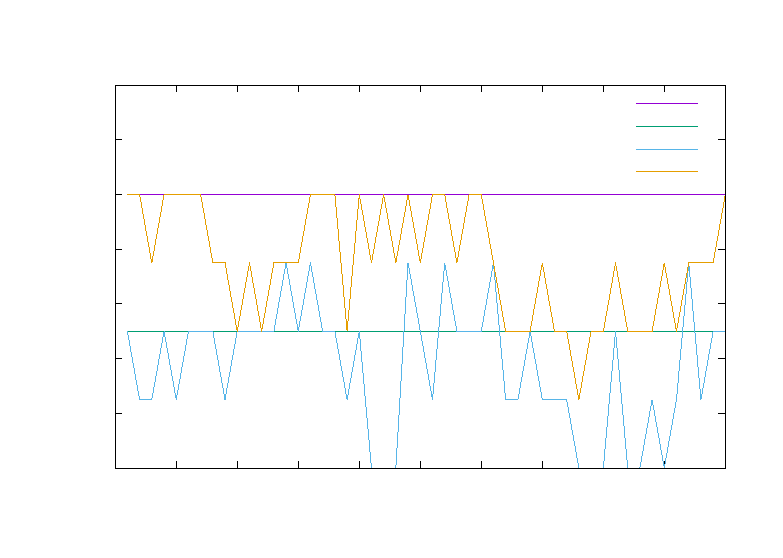
\includegraphics[width={360.00bp},height={252.00bp}]{pairwise}}%
    \gplfronttext
  \end{picture}%
\endgroup
 
\end {center}
\caption{Results from four static 50 round tournaments with
  neighbourhood voting.  3-TFT refers to 3 tit-for-tat agents that
  start cooperating; note that they continue to cooperate.  2-TFT+D
  refers to two tit-for-tat agents with an agent that always defects;
  this leads to system where the TFT agents collaborate with each
  other and defect against the defecting agent.  2-TFT-E+D refers to
  two tit-for-tat agents with 10\% exploration and an always defect
  agent; this leads to a system where the TFT agents have some
  collaboration but mostly defect.  2-TFT-E+C refers to two
  tit-for-tat agents with 10\% exploration and an agent that always
  cooperates; the TFT agents mostly collaborate, but there is some
  defection. }
  \label{figStaticTwoVotes}
\end {figure}


The TFT agents initially cooperate, so they remain in the fully cooperative
state.  When the two TFT agents work with a collaborative agent, they also
always cooperate.  When they work the always defect agent, they initially
collaborate, but then decide to repeatedly defect against the defector.  This
leads to a lower average payout, but is still largely collaborative.  When
exploration is included, the TFT-E agents occasionally defect, and then
punish the other defecting agent.  This leads to an oscillation that tends
toward cooperation.  


The second set of simulations uses pairwise voting.  The results
are shown in figure \ref {figStaticOneVote}. The same four sets
of agents, using static policies, are used.  The three TFT agents continue
to collaborate, as do the two TFT agents with the always collaborate agent
(not shown in figure \ref {figStaticOneVote}).
However, the TFT agents with the always defect initially vote to collaborate,
but then quickly move to always defect.  They descend into the tragic valley.
The TFT-E system is more likely to move up and down, but also tends toward
but also largely hovers about both defecting.    

\begin{figure}
\begin{center}
% GNUPLOT: LaTeX picture with Postscript
\begingroup
  \makeatletter
  \providecommand\color[2][]{%
    \GenericError{(gnuplot) \space\space\space\@spaces}{%
      Package color not loaded in conjunction with
      terminal option `colourtext'%
    }{See the gnuplot documentation for explanation.%
    }{Either use 'blacktext' in gnuplot or load the package
      color.sty in LaTeX.}%
    \renewcommand\color[2][]{}%
  }%
  \providecommand\includegraphics[2][]{%
    \GenericError{(gnuplot) \space\space\space\@spaces}{%
      Package graphicx or graphics not loaded%
    }{See the gnuplot documentation for explanation.%
    }{The gnuplot epslatex terminal needs graphicx.sty or graphics.sty.}%
    \renewcommand\includegraphics[2][]{}%
  }%
  \providecommand\rotatebox[2]{#2}%
  \@ifundefined{ifGPcolor}{%
    \newif\ifGPcolor
    \GPcolortrue
  }{}%
  \@ifundefined{ifGPblacktext}{%
    \newif\ifGPblacktext
    \GPblacktexttrue
  }{}%
  % define a \g@addto@macro without @ in the name:
  \let\gplgaddtomacro\g@addto@macro
  % define empty templates for all commands taking text:
  \gdef\gplbacktext{}%
  \gdef\gplfronttext{}%
  \makeatother
  \ifGPblacktext
    % no textcolor at all
    \def\colorrgb#1{}%
    \def\colorgray#1{}%
  \else
    % gray or color?
    \ifGPcolor
      \def\colorrgb#1{\color[rgb]{#1}}%
      \def\colorgray#1{\color[gray]{#1}}%
      \expandafter\def\csname LTw\endcsname{\color{white}}%
      \expandafter\def\csname LTb\endcsname{\color{black}}%
      \expandafter\def\csname LTa\endcsname{\color{black}}%
      \expandafter\def\csname LT0\endcsname{\color[rgb]{1,0,0}}%
      \expandafter\def\csname LT1\endcsname{\color[rgb]{0,1,0}}%
      \expandafter\def\csname LT2\endcsname{\color[rgb]{0,0,1}}%
      \expandafter\def\csname LT3\endcsname{\color[rgb]{1,0,1}}%
      \expandafter\def\csname LT4\endcsname{\color[rgb]{0,1,1}}%
      \expandafter\def\csname LT5\endcsname{\color[rgb]{1,1,0}}%
      \expandafter\def\csname LT6\endcsname{\color[rgb]{0,0,0}}%
      \expandafter\def\csname LT7\endcsname{\color[rgb]{1,0.3,0}}%
      \expandafter\def\csname LT8\endcsname{\color[rgb]{0.5,0.5,0.5}}%
    \else
      % gray
      \def\colorrgb#1{\color{black}}%
      \def\colorgray#1{\color[gray]{#1}}%
      \expandafter\def\csname LTw\endcsname{\color{white}}%
      \expandafter\def\csname LTb\endcsname{\color{black}}%
      \expandafter\def\csname LTa\endcsname{\color{black}}%
      \expandafter\def\csname LT0\endcsname{\color{black}}%
      \expandafter\def\csname LT1\endcsname{\color{black}}%
      \expandafter\def\csname LT2\endcsname{\color{black}}%
      \expandafter\def\csname LT3\endcsname{\color{black}}%
      \expandafter\def\csname LT4\endcsname{\color{black}}%
      \expandafter\def\csname LT5\endcsname{\color{black}}%
      \expandafter\def\csname LT6\endcsname{\color{black}}%
      \expandafter\def\csname LT7\endcsname{\color{black}}%
      \expandafter\def\csname LT8\endcsname{\color{black}}%
    \fi
  \fi
    \setlength{\unitlength}{0.0500bp}%
    \ifx\gptboxheight\undefined%
      \newlength{\gptboxheight}%
      \newlength{\gptboxwidth}%
      \newsavebox{\gptboxtext}%
    \fi%
    \setlength{\fboxrule}{0.5pt}%
    \setlength{\fboxsep}{1pt}%
    \definecolor{tbcol}{rgb}{1,1,1}%
\begin{picture}(7200.00,5040.00)%
    \gplgaddtomacro\gplbacktext{%
      \csname LTb\endcsname%%
      \put(814,704){\makebox(0,0)[r]{\strut{}$0$}}%
      \put(814,1229){\makebox(0,0)[r]{\strut{}$0.2$}}%
      \put(814,1754){\makebox(0,0)[r]{\strut{}$0.4$}}%
      \put(814,2279){\makebox(0,0)[r]{\strut{}$0.6$}}%
      \put(814,2804){\makebox(0,0)[r]{\strut{}$0.8$}}%
      \put(814,3329){\makebox(0,0)[r]{\strut{}$1$}}%
      \put(814,3854){\makebox(0,0)[r]{\strut{}$1.2$}}%
      \put(814,4379){\makebox(0,0)[r]{\strut{}$1.4$}}%
      \put(946,484){\makebox(0,0){\strut{}$0$}}%
      \put(1532,484){\makebox(0,0){\strut{}$5$}}%
      \put(2117,484){\makebox(0,0){\strut{}$10$}}%
      \put(2703,484){\makebox(0,0){\strut{}$15$}}%
      \put(3289,484){\makebox(0,0){\strut{}$20$}}%
      \put(3875,484){\makebox(0,0){\strut{}$25$}}%
      \put(4460,484){\makebox(0,0){\strut{}$30$}}%
      \put(5046,484){\makebox(0,0){\strut{}$35$}}%
      \put(5632,484){\makebox(0,0){\strut{}$40$}}%
      \put(6217,484){\makebox(0,0){\strut{}$45$}}%
      \put(6803,484){\makebox(0,0){\strut{}$50$}}%
    }%
    \gplgaddtomacro\gplfronttext{%
      \csname LTb\endcsname%%
      \put(5816,4206){\makebox(0,0)[r]{\strut{}3-TFT}}%
      \csname LTb\endcsname%%
      \put(5816,3986){\makebox(0,0)[r]{\strut{}2-TFT+D}}%
      \csname LTb\endcsname%%
      \put(5816,3766){\makebox(0,0)[r]{\strut{}2-TFT-E+D}}%
      \csname LTb\endcsname%%
      \put(5816,3546){\makebox(0,0)[r]{\strut{}2-TFT-E+C}}%
      \csname LTb\endcsname%%
      \put(209,2541){\rotatebox{-270.00}{\makebox(0,0){\strut{}Cooperation}}}%
      \put(3874,154){\makebox(0,0){\strut{}Round}}%
      \put(3874,4709){\makebox(0,0){\strut{}Average Cooperation by Round with Neighbourhood Voting}}%
    }%
    \gplbacktext
    \put(0,0){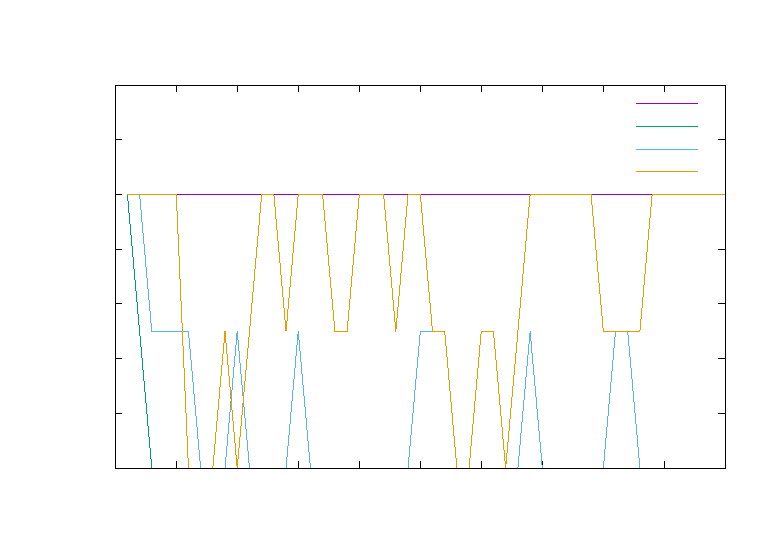
\includegraphics[width={360.00bp},height={252.00bp}]{neighbourhood}}%
    \gplfronttext
  \end{picture}%
\endgroup
 
\end {center}
\caption{Results from four 50 round tournaments with static agents
  with neighbourhood voting.  3-TFT refers to 3 tit-for-tat agents
  that start cooperating; they continue to cooperate.  2-TFT+D refers
  to two tit-for-tat agents with an agent that always defects; this
  quickly descends to no cooperation.  2-TFT-E+D refers to two
  tit-for-tat agents with 10\% exploration and an always defect agent;
  this system has some cooperations but mostly defects; note that it
  defects more than when there is pairwise voting.  2-TFT-E+C refers
  to two tit-for-tat agents with 10\% exploration and an agent that
  always cooperates; this cooperates about half the time, which is
  less than when there is pairwise voting.}
  \label{figStaticOneVote}
\end {figure}


The reason behind this is that the reward space for each agent tends
toward the positive when there is pairwise voting.  Each agent can
punish particular defectors and reward particular collaborators.  This
is why the agents can all get better results and ascend the
collaborative hill.  On the other hand, with neighbourhood voting,
each agent can only reward or punish in aggregate.  The reward structure is
that each agent does better by defecting, and any collaboration tends to
give worse immediate results.  This reward space and the agents' ability
to only weakly influence other agents draws the agents into the Tragic
Valley where agents do not cooperate.

\section {Reinforcement Learning Agents}

The authors were suprised that they found no papers explicitly stating
that pairwise voting led to largely good performance.  However, this
may be due to pairwise voting really just being  $(N-1)*(N-2)$ individual
tournaments.  Thus, the original work on the two person Prisoner's Dilemma
holds.

undone end

3.  **pTFT-Threshold - N-Person Model:** An enhancement to pTFT. Agents cooperate if the previous round's overall group cooperation rate was 50\% or higher. If below 50\%, they revert to the standard pTFT rule (cooperating probabilistically based on the exact sub-50\% rate).

\subsection{Experimental Parameters and Variations}
Our experiments systematically varied several factors:

1.  **Agent Compositions:** We tested populations of 3 and 5 agents, with mixes such as:
    *   Purely TFT-type agents (e.g., 3 TFTs).
    *   Mixed populations (e.g., 2 TFTs and 1 AllD; 2 TFTs and 3 AllDs).
2.  **Exploration Rate (Error):** Agents had a 0\% or 10\% chance of making a move contrary to their intended strategy. This introduces stochasticity and tests the robustness of strategies.
3.  **Episodic Resets (Pairwise Model Only):** For some pairwise experiments, interactions were divided into 10 "episodes" of 10 rounds each (totaling 100 rounds per pair). At the end of each episode, TFT agents would "forget" their opponent's last move, effectively starting the next episode with a clean slate (i.e., cooperating). Non-episodic pairwise runs consisted of a single 100-round interaction per pair.
4.  **Rounds:** Pairwise interactions involved 100 total rounds per pair. N-Person simulations ran for 200 rounds.

\subsection{Key Metrics for Evaluation}
To assess outcomes, we focused on:

1.  **Agent Score:** The cumulative payoff an agent received throughout all its interactions. This reflects individual success.
2.  **Cooperation Rate:** For an individual agent, this is the percentage of times it chose to cooperate out of its total moves. This indicates an agent's behavioral tendency.
3.  **Overall Cooperation Rate:**
    *   For Pairwise: The average cooperation rate across all moves made by all agents in all their dyadic games.
    *   For N-Person: The average per-round cooperation rate of the entire group over the simulation. This reflects the collective group behavior.

    By analyzing these metrics across the varied experimental conditions, we aim to elucidate how interaction structure, agent strategies, and environmental factors combine to shape the emergence and stability of cooperation, leading to the contrasting dynamics of the Reciprocity Hill and the Tragedy Valley.
    

r specific
experimental configurations, and the metrics used (Section
\ref{sec:framework_and_methodology}). The core findings contrasting
interaction structures and adaptive strategies are presented in
Section \ref{sec:results_discussion_valley_hill}. Finally, we discuss
the broader implications (Section \ref{sec:general_discussion}) and
conclude with future research directions (Section
\ref{sec:conclusion}).


This extension introduces significant complexities:
\begin{itemize}
    \item \textbf{Diffused Responsibility and Payoffs:} The impact of a single agent's cooperative or defective action is spread across the group, diluting the direct consequences felt by any one individual.
    \item \textbf{Obscured Reciprocity:} It becomes harder to identify and respond to specific cooperators or defectors, making direct tit-for-tat like reciprocity challenging.
    \item \textbf{Increased Temptation to Free-Ride:} With many participants, an individual might be more tempted to defect, hoping to benefit from others' cooperation without contributing.
\end{itemize}

These complexities often lead rational, self-interested agents in N-IPD scenarios towards a "Tragedy Valley" of widespread defection, a concept echoing Hardin's "Tragedy of the Commons" \cite{Hardin1968}. 
Our computational explorations using agent-based models (ABMs) with standard reinforcement learning (RL) agents consistently confirm this pessimistic outcome in certain N-IPD structures. This paper investigates the cognitive and structural conditions that allow learning agents to escape this valley and, in more favorable settings, ascend a "Reciprocity Hill" where cooperation can flourish.

We present \texttt{npdl}, an agent-based simulation framework, to explore these dynamics. Our central argument is that the emergence of cooperation in the N-IPD is not solely dependent on sophisticated learning algorithms but is critically shaped by (a) the agents' ability to perceive \textbf{context} from their social environment, (b) the inherent \textbf{adaptability} of their learning mechanisms, and (c) the fundamental **interaction structure** of the dilemma itself.

The key takeaways from our investigation are:
\begin{enumerate}
    \item \textbf{The "Tragedy Valley" vs. "Reciprocity Hill" (Interaction Structure - T1):} The structure of agent interactions is paramount.
        \begin{itemize}
            \item In N-IPD \textit{neighbourhood models}, where an agent's single choice affects a diffuse group payoff, most learning algorithms (including standard RL and simpler reactive strategies like Tit-for-Tat) tend to descend into the "Tragedy Valley" of defection.
            \item In contrast, N-IPD \textit{pairwise models}, where each agent effectively makes $N-1$ choices by engaging in distinct 2-player games with all others, direct reciprocity is clear. This structure facilitates climbing a "Reciprocity Hill" where cooperation is more readily established and maintained.
        \end{itemize}
    \item \textbf{Context is Crucial for Escaping the Valley (Cognitive Prerequisite - T2):} For agents operating in the challenging neighbourhood model, perceiving local social context (e.g., the proportion of cooperating neighbours) is a vital first step to avoid immediate and total defection.
    \item \textbf{Adaptive MARL Can Navigate the Valley (Learning Mechanism - T3):} Even within the difficult neighbourhood model, advanced Multi-Agent Reinforcement Learning (MARL) algorithms—particularly those incorporating optimism (like Hysteretic-Q) or adaptive learning rates (like Wolf-PHC)—can enable agents to learn resilient cooperative strategies and achieve high, sustained cooperation. Standard RL often fails where these succeed.
\end{enumerate}


\begin{itemize}
    \item \textbf{Dominance of Defection:} For any individual, defecting yields a higher personal payoff than cooperating, regardless of how many others cooperate. Formally, if an agent considers switching from cooperate to defect, its payoff increases: $P_D(n_c) > P_C(n_c+1)$ where $n_c$ is the number of *other* cooperators (if the agent defects) versus $n_c+1$ (if the agent cooperates).
    \item \textbf{Deficient Equilibrium:} Universal cooperation yields a better payoff for every individual than universal defection: $P_C(N) > P_D(0)$.
\end{itemize}
This inherent conflict between individual rationality (defect) and collective benefit (cooperate) often leads to the "Tragedy of the Commons" \cite{Hardin1968}, where shared resources are depleted. Our concept of the "Tragedy Valley" directly reflects this gravitational pull towards mutual defection observed in N-IPD simulations.

\section{Simulation Framework, Experimental Setup, and Metrics}
\label{sec:framework_and_methodology} % Replaces your old Chapter 3


\section{The Dichotomy of Reciprocity: Navigating the Tragedy Valley and Ascending the Reciprocity Hill}
\label{sec:results_discussion_valley_hill} % This is your new chapter 3, now framed as results/discussion

The Iterated Prisoner's Dilemma (IPD) has long served as a crucible for understanding cooperation. Axelrod's seminal work demonstrated the remarkable success of simple reciprocal strategies like Tit-for-Tat (TFT) in fostering mutual benefit in two-player encounters. However, the transition from dyadic interactions to scenarios involving multiple agents—the N-Person IPD (N-IPD)—unveils a dramatically altered strategic landscape. This section delves into a fundamental dichotomy observed in our simulations: the "Reciprocity Hill," where direct, pairwise interactions allow simple reciprocity to flourish, and the "Tragedy Valley," a perilous domain where the same reciprocal logic, when applied in standard N-Person neighbourhood models, often leads to a swift collapse of cooperation.

We will explore how the very structure of interaction dictates the fate of cooperative strategies. Using our agent-based modeling framework (detailed in Section \ref{sec:framework_and_methodology}), we demonstrate how TFT, a champion of cooperation in pairwise settings, struggles when its principles are translated to the N-Person context without significant adaptation. We then investigate the impact of environmental noise (exploration/error) and strategic modifications—such as episodic memory resets in pairwise games and a threshold-based decision rule in N-Person games—on navigating these distinct landscapes.

\subsection{The Reciprocity Hill: Pairwise Interactions and the Power of Direct Accountability}
In the classic pairwise IPD, the path to cooperation, or the "Reciprocity Hill," is paved with clarity and direct accountability. When two agents interact repeatedly, several factors contribute to cooperative success. An agent's action (cooperate or defect) directly impacts the other, and the payoff received is an immediate consequence of this dyadic choice, establishing a clear cause and effect. Strategies like TFT can precisely mirror an opponent's previous move; cooperation is rewarded with cooperation, and defection is met with defection, all targeted at the specific individual involved, which prevents "punishing" innocent bystanders. Furthermore, TFT's willingness to cooperate after an opponent's defection (if the opponent returns to cooperation) allows for recovery from isolated defections or misunderstandings, facilitating forgiveness and re-engagement.

Our simulations starkly confirm this. In scenarios with 0\% exploration, groups of three TFT agents in the pairwise model consistently achieved perfect cooperation (1.00 overall cooperation rate), with all agents maximizing their potential scores (e.g., 600 points). Even when introducing a single Always Defect (AllD) agent among two TFTs, the TFT agents maintained perfect cooperation with each other while quickly learning to defect against the AllD after its initial defection. The TFTs still achieved high scores (e.g., 399 points), demonstrating their robustness in isolating defectors while preserving mutual benefit with cooperators. This ability to selectively engage allows TFT to thrive on the Reciprocity Hill.

\subsection{The Tragedy Valley: N-Person Interactions and the Perils of Diffused Reciprocity}
The N-Person IPD, particularly in a "neighbourhood" or "group payoff" model where an agent's single choice affects and is affected by the collective, presents a starkly different challenge. Here, simple reciprocity often leads agents into a "Tragedy Valley" of mutual defection. The key difficulties include diffused responsibility and payoffs, where the impact of an individual's action is spread across the group, making it hard to assign credit or blame. Reciprocity becomes obscured: who should a TFT-like agent retaliate against if the group outcome is poor? If it defects, it punishes cooperators and defectors alike. A direct, one-to-one mirroring is impossible. Finally, there is an increased temptation to free-ride, as an individual might defect hoping to benefit from others' cooperation without their own defection having an obvious negative consequence on any single player.

Our simulations employed a Probabilistic Tit-for-Tat (pTFT) for the N-Person model, which cooperates based on the previous round's overall cooperation ratio in the group.
With 0\% exploration, in a group of three pTFT agents, cooperation was initially perfect, leading to optimal scores (600 points), mirroring the pairwise outcome without disruptors.
However, introducing a single AllD agent drastically changed the dynamic. With two pTFTs and one AllD, the initial cooperation ratio (ignoring exploration) would be 2/3. In subsequent rounds, pTFTs would cooperate with a ~67\% chance. If one pTFT agent defected (due to this probability or the AllD's continued defection), the overall cooperation ratio would drop further. Our simulations showed a rapid descent into the Tragedy Valley: the overall cooperation rate plummeted to approximately 0.01, with AllD achieving the highest score (e.g., around 206-210 points) by exploiting the initial cooperative overtures and subsequent confusion. The pTFT agents, unable to target the defector or coordinate effectively, ended up with significantly lower scores (around 200-203 points). With an even higher proportion of defectors (2 pTFTs, 3 AllDs), the collapse of cooperation was even more pronounced and immediate, with overall cooperation near 0\%. This demonstrates that the direct translation of TFT's reciprocal logic via pTFT is insufficient to escape the Tragedy Valley in the N-Person model when faced with persistent defectors; the very structure diffuses the information needed for simple reciprocity to gain a foothold.

\subsection{Navigating the Landscapes: The Role of Noise, Memory, and Strategic Adaptation}
The introduction of environmental noise (exploration/error) and specific strategic adaptations further highlights the differences between these two landscapes and reveals pathways to either fortify cooperation or attempt escape from defection traps.

\subsubsection{The Impact of Exploration (Error)}
An exploration rate (e.g., 10\%) introduces a chance for agents to make a move contrary to their strategy. This "noise" has distinct consequences.
On the Reciprocity Hill (Pairwise), among pure TFT groups, exploration significantly degrades cooperation (e.g., from 1.00 to ~0.40-0.54 overall cooperation), as errors can initiate prolonged cycles of mutual defection. When AllD agents are present, exploration can sometimes benefit them or harm them, while TFTs also suffer from their own errors.
In the Tragedy Valley (N-Person), among pure pTFT groups, exploration also reduces cooperation (e.g., from 1.00 to ~0.48 overall). An erroneous defection lowers the group cooperation ratio, making subsequent cooperation by other pTFTs less likely. With AllD agents, exploration makes the already dire situation for pTFTs slightly more chaotic. AllD's own errors might momentarily boost the cooperation ratio, giving pTFTs a brief, often futile, chance to cooperate more, but overall cooperation remains very low (around 0.24-0.29 with 2 pTFTs/1 AllD).

\subsubsection{Mending Fences on the Hill: Episodic Resets in Pairwise TFT}
To counteract the negative impact of error-induced defection spirals in pairwise interactions, we introduced an "episodic" mode where TFT agents reset their memory of an opponent's last move after a set number of rounds (e.g., 10 episodes of 10 rounds).
With 0\% exploration, this led to AllD scoring higher (e.g., 280 vs 208) because TFTs repeatedly "forgave" and cooperated at the start of each new episode. TFTs also cooperated slightly more overall when interacting with AllD alongside another TFT (0.55 vs 0.51 agent cooperation rate).
With 10\% exploration, in pure TFT groups, episodic resets were highly beneficial. Overall cooperation jumped from approximately 0.40-0.54 (non-episodic) to 0.66-0.69 (episodic). By "forgetting" past grievances, agents could more easily break out of retaliation cycles. With AllD agents, episodic resets still helped TFTs maintain higher cooperation levels compared to non-episodic noisy runs, but AllD still benefited significantly. Episodic memory resets act as a mechanism to increase the "forgiveness" aspect of the Reciprocity Hill, making it more resilient to noise among cooperators, but also more vulnerable to exploitation by defectors.

\subsubsection{Seeking an Escape from the Valley: The pTFT-Threshold Variant in N-Person}
Recognizing pTFT's vulnerability, we introduced the pTFT-Threshold variant: cooperate deterministically if the previous round's overall cooperation rate is >= 50\%, and probabilistically (scaled) if below 50\%.
With 0\% exploration, this strategy yielded a striking result with 2 pTFT-Threshold agents and 1 AllD: the TFTs maintained perfect mutual cooperation (1.00 individual rate). The initial 2/3 cooperation ratio kept them above the 0.5 threshold, creating a stable cooperative equilibrium among them. AllD, defecting consistently, received the Temptation payoff and scored very high (1000 points), while TFTs scored 300 points each. This demonstrates a successful, albeit costly for TFTs against AllD, escape from the Tragedy Valley for the cooperative subgroup. With more AllDs (2 TFTs, 3 AllDs), the initial cooperation (2/5 = 0.4) was below the threshold, and cooperation quickly eroded (around 0.03 overall), similar to standard pTFT.
With 10% exploration, in pure pTFT-Threshold groups, cooperation was remarkably high (around 0.86-0.87 overall), demonstrating strong resilience to noise. With 2 pTFT-Threshold agents and 1 AllD, overall cooperation was significantly higher (around 0.54) than with standard pTFT (around 0.24-0.29). AllD still scored highest. With 2 TFTs and 3 AllDs, pTFT-Threshold still performed better than pTFT (around 0.25 vs 0.12-0.15 overall cooperation), but the high number of defectors made sustained group cooperation difficult. The pTFT-Threshold offers a more robust heuristic for N-Person scenarios, allowing conditional cooperators to better coordinate and resist the downward pull of defections or moderate noise, effectively building small "foothills of reciprocity" within the broader Tragedy Valley.

\subsubsection{The Unwavering Weight of Defection: Impact of Agent Compositions}
Across all models and variations, increasing the proportion of AllD agents consistently made cooperation more challenging and less rewarding for TFT-type agents. In Pairwise interactions, while TFTs could still maintain cooperation with each other, their overall scores and cooperation rates diminished due to more interactions with AllDs. In N-Person settings, a higher density of AllDs quickly overwhelmed both pTFT and pTFT-Threshold strategies, dragging the group deep into the Tragedy Valley, as the threshold for pTFT-Threshold becomes harder to reach and sustain.

\subsection{Synthesis: Interaction Structure as the Primary Determinant}
Our comprehensive experiments illuminate a critical insight: the structure of interaction is a primary determinant of whether simple reciprocal strategies lead to a "Reciprocity Hill" of sustained cooperation or a "Tragedy Valley" of mutual defection. Pairwise interactions, with their direct accountability, naturally support TFT-like reciprocity. Standard N-Person neighbourhood models, with their diffused responsibility and obscured feedback, inherently undermine it. Strategic adaptations can modulate these landscapes but are often secondary to the fundamental influence of the interaction structure itself.


\section{General Discussion}
\label{sec:general_discussion} % This section can be expanded with your MARL agent comparisons and broader implications from your original draft.
Our experimental results, focusing on reactive strategies and their adaptations, shed light on the critical factors influencing cooperation in the N-Person Iterated Prisoner's Dilemma. The "Tragedy Valley" and "Reciprocity Hill" metaphors effectively capture the divergent outcomes based on interaction structure.

The consistent failure of simple reciprocal logic (pTFT) in the N-Person neighbourhood model when defectors are present, contrasted with its success in pairwise settings, underscores the profound impact of structural properties like accountability and clarity of feedback. While advanced MARL algorithms like Hysteretic-Q and Wolf-PHC (as explored in related work \cite{TcaciHuyck2023Hysteretic, TcaciHuyck2023WoLFPHC}) can achieve high cooperation even in difficult N-IPD neighbourhood models through more sophisticated learning, our findings with simpler strategies highlight the baseline challenges. The pTFT-Threshold variant demonstrates that even relatively simple cognitive enhancements, allowing agents to react to a critical mass of cooperation, can significantly improve outcomes in N-Person settings.

The effectiveness of episodic memory resets in mitigating error-induced defection spirals in pairwise TFT interactions further points to the importance of mechanisms that allow for "re-setting" relationships, especially in noisy environments.

These findings collectively suggest that understanding and promoting cooperation in complex multi-agent systems requires a multifaceted approach. Attention must be paid not only to individual agent learning capacities and cognitive heuristics but also, critically, to the design of the interaction structures themselves. Facilitating clearer feedback loops and more direct accountability, where possible, may be key to helping agents ascend Reciprocity Hills rather than descend into Tragedy Valleys.

Limitations of this study include the abstraction of agent cognition (using rule-based strategies rather than full RL for the core comparisons here) and the focus on specific payoff parameters. Future work will continue to explore the comparative dynamics of neighbourhood versus pairwise models with a wider range of learning agents and environmental complexities.

\section{Conclusion}
\label{sec:conclusion}
This paper demonstrated that while N-IPD in neighbourhood models often leads to a "Tragedy Valley" for simple reciprocal strategies, the interaction structure is critical. Pairwise models, facilitating a "Reciprocity Hill," make cooperation more accessible for strategies like Tit-for-Tat. Adaptations such as episodic memory resets in pairwise games and threshold-based decision rules in N-Person games can significantly modulate cooperative outcomes, especially in the presence of noise. Our \texttt{npdl} framework enables these systematic explorations, highlighting that both agent cognition and, crucially, the structure of their interactions, are key to understanding and promoting cooperation in complex multi-agent systems. Future work will further investigate these dynamics with more diverse learning algorithms and scenarios.


% --- Bibliography ---
\bibliographystyle{ieeetr} % Using a standard IEEE transaction style (numbered)
\bibliography{prisoners}   % Your .bib file is named prisoners.bib

% --- Appendix (Optional - if you want to keep your original Chapter 3/Results) ---
\begin{subappendices} % Using subappendices from appendix package
\label{app:original_results}


\end{subappendices}


\end{document}
